\begin{minipage}[t]{180mm}
\fcolorbox{black}{white}{
\begin{minipage}[b]{30mm}

\includegraphics[width=0.5\linewidth]{unflogo.pdf}
\end{minipage}
\begin{minipage}[b]{100mm}
\Huge \textbf{UNF NEWZ} \\
\Large -- Søvn og retsstavning er overvurderet! 
\end{minipage}
\begin{minipage}[b]{50mm}
\Large Onsdag 17.07.2015 \\
\normalsize Redigeret i \LaTeX\ af \\ SOM, MGS, MMN, SABH
\end{minipage}
}
\end{minipage}



\begin{minipage}[b]{0.95\linewidth}
\begin{minipage}[t]{0.47\textwidth}
\vspace{3mm}
\section*{Koordinativ Resolution}

Paa Campens derom nedlagte allerunderdanigste Forestilling har det under den femtende i Ormemaaneden i det tohundredeseksogtredivte Aar behaget mig, Campens Koordinator af Gauss Naade, Eulers Husholder og Galois ydmyge Efterfølger, at afstaa al Eierskab i Husalfen i en begrænset Periode mellem Solopgang og Solnedgang denne femtende i Ormemaaneden i det tohundredeseksogtredivte Aar. Dette vil dog ingenlunde begrænse Husalfens Forpligtelser, hverken over for Campen eller over for dens Tjenestemænd. Under mit Eierskabs Fravær paalægges Ansvaret for Tilsynet over Husalfens Ve, Vel og Opførsel det til dette Formaal nedsatte Konsistorium, bestaaende af de Arrangører paa Campen hvis upaaklagelige Ry gør dem egnet til Hvervet.

{\flushright\emph{Morten Grue Sørensen, Koordinator af Gauss naade }}


\section*{Campens forfatningsretlige status}
Det har i årevis været et omdiskuteret emne blandt lærde i sommerskoleforfatningsvidenskab om campen som organisation skal anses som \emph{corporation sole} eller som \emph{corporation aggregate}. I lighed med forholdene der gælder for den britiske krone er førstnævnte den mest udbredte interpretation og tydeligvis også den der ligger til grund for ovenstående resolution. 

\end{minipage}
\hfill\begin{minipage}[t]{0.47\textwidth}

\vspace{1mm}
\tikzstyle{mybox} = [draw=white, fill=blue!20, very thick,
    rectangle, rounded corners, inner sep=10pt, inner ysep=20pt]
\tikzstyle{fancytitle} =[fill=red, text=white]

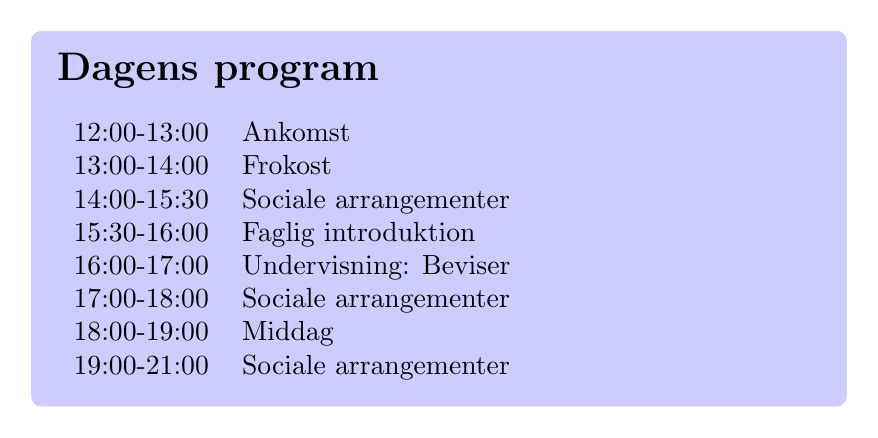
\begin{tikzpicture}
\node [mybox] (box){%
\begin{minipage}{0.80\textwidth}
\vspace{-4mm}\section*{Dagens program}
\begin{tabular}{ll}
12:00-13:00 & Ankomst \\
13:00-14:00 & Frokost \\
14:00-15:30 & Sociale arrangementer \\
15:30-16:00 & Faglig introduktion \\
16:00-17:00 & Undervisning: Beviser \\
17:00-18:00 & Sociale arrangementer \\
18:00-19:00 & Middag \\
19:00-21:00 & Sociale arrangementer \\
\end{tabular}
\vspace{-4mm}
\end{minipage}
};
\end{tikzpicture}%



\end{minipage}
\end{minipage}
